% =====================================================================
% Слайд 2 — Проблема
% =====================================================================
\begin{frame}{Проблема: аккомпаниатор, а не фонограмма}
  \small
  \begin{columns}[T,onlytextwidth]
    \column{0.46\textwidth}
    \vspace{0.4em}
    \begin{itemize}\setlength{\itemsep}{0.45em}
      \item Солисту-пианисту перед концертом нужно репетировать
            \textbf{с оркестром}.
      \item Живой оркестр на каждую репетицию --- недоступно
            (бюджет, время, организация).
      \item Фиксированная фонограмма не работает: она не
            подстраивается под темп, артикуляцию и \emph{rubato}
            солиста.
      \item \rlhi{Цель:} виртуальный оркестр, который играет
            заданное сопровождение и подстраивается под солиста
            \textbf{в реальном времени}.
    \end{itemize}

    \column{0.54\textwidth}
    \centering
    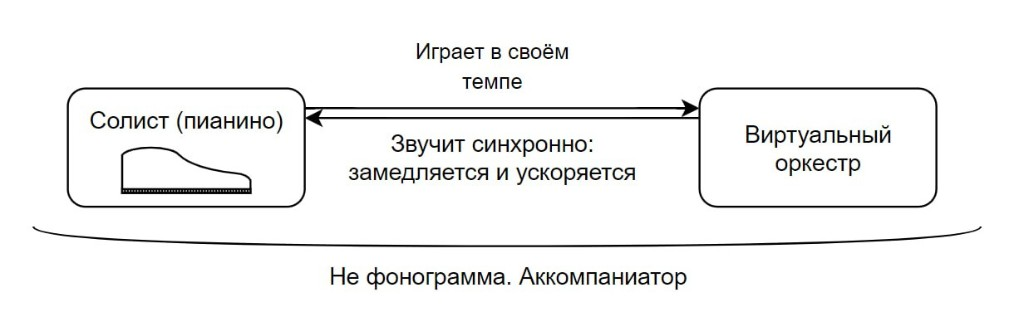
\includegraphics[width=\linewidth]{figures/png/world_view.png}
  \end{columns}
\end{frame}
